\documentclass[11pt]{article}

%\usepackage{palatino}

\usepackage[utf8]{inputenc}
\usepackage[T1]{fontenc}
% Chivo como en las diapositivas o Fira Sans?
%\usepackage[familydefault,regular]{Chivo}
\usepackage[sfdefault,scaled=.85]{FiraSans}
\usepackage{newtxsf}
\usepackage[spanish]{babel}
\setlength{\parindent}{0pt}
\usepackage{amssymb}
\usepackage{amsmath}
\usepackage{wasysym}
\usepackage[x11names, rgb, html]{xcolor}
\usepackage{graphics}
\usepackage{caption}
\usepackage{lipsum}
\usepackage{float}
\usepackage{adjustbox}
\usepackage{geometry}
\usepackage[scaled=.85]{FiraMono}  

\geometry{left=3cm,right=3cm,top=3cm,bottom=3cm,headheight=1cm,headsep=0.5cm} 


%%% PGFPLOTSTABLE

\usepackage{pgfplotstable}

%%% COLORES


%% Colores de Solarized

\definecolor{sbase03}{HTML}{002B36}
\definecolor{sbase02}{HTML}{073642}
\definecolor{sbase01}{HTML}{586E75}
\definecolor{sbase00}{HTML}{657B83}
\definecolor{sbase0}{HTML}{839496}
\definecolor{sbase1}{HTML}{93A1A1}
\definecolor{sbase2}{HTML}{EEE8D5}
\definecolor{sbase3}{HTML}{FDF6E3}
\definecolor{syellow}{HTML}{B58900}
\definecolor{sorange}{HTML}{CB4B16}
\definecolor{sred}{HTML}{DC322F}
\definecolor{smagenta}{HTML}{D33682}
\definecolor{sviolet}{HTML}{6C71C4}
\definecolor{sblue}{HTML}{268BD2}
\definecolor{scyan}{HTML}{2AA198}
\definecolor{sgreen}{HTML}{859900}

%% Colores del documento

\definecolor{text}{RGB}{78,78,78}
\definecolor{accent}{RGB}{129, 26, 24}

%%% LISTINGS

\usepackage{listingsutf8}

%% Las tildes

\lstset{
  inputencoding=utf8/latin1
}

%% Colores de Solarized para listings

\lstset{
  % How/what to match
  % sensitive=true,
  language=C++,
  % Border (above and below)
  frame=lines,
  % Line number
  numbers=left,
  % Extra margin on line (align with paragraph)
  xleftmargin=\parindent,
  % Put extra space under caption
  belowcaptionskip=1\baselineskip,
  % Colors
  % backgroundcolor=\color{sbase3},
  basicstyle=\footnotesize\ttfamily\color{sbase00},
  keywordstyle=\color{scyan},
  commentstyle=\color{sbase1},
  stringstyle=\color{sblue},
  numberstyle=\color{sbase01},
  identifierstyle=\color{smagenta},
  % Break long lines into multiple lines?
  breaklines=true,
  % Show a character for spaces?
  showstringspaces=false,
  tabsize=2
}


\title{Algorítmica: práctica 3 \\ \large Recubrimiento de un grafo no dirigido\\ \vspace{0.2em}Grupo 2}
\author{Sofía Almeida Bruno \and Antonio Coín Castro \and María Victoria Granados Pozo \and Miguel Lentisco Ballesteros \and José María Martín Luque}
\date{\today}

\begin{document}
\maketitle

\newpage

\section*{Introducción}

Dado un grafo no dirigido G=(V,E), un conjunto U $\subseteq$ V es un recubrimiento de G si cada arista en E incide en, al menos, un vértice o nodo de U. Nuestro problema consiste en encontrar un recubrimiento minimal del grafo G, esto es, un recubrimiento con el menor número posible de nodos. La solución que proporcionamos es el conjunto de nodos que forman el recubrimiento junto con el coste (número de nodos). 

\begin{figure}[H]
	\caption{Ejemplo de grafo. Los nodos más oscuros forman el recubrimiento}
	\centering 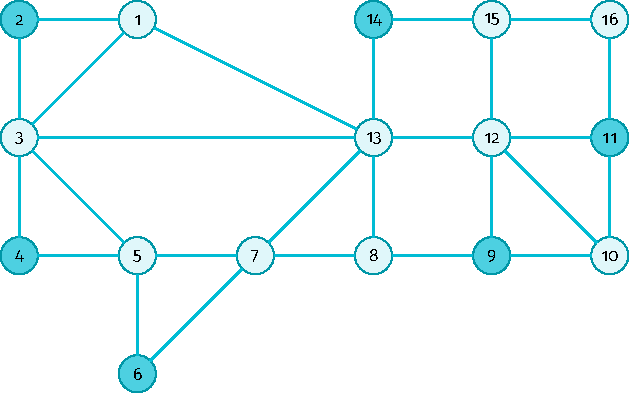
\includegraphics{./img/grafo.pdf}
\end{figure}

\section*{Algoritmo Greedy}

En primer lugar, vamos a mostrar las componentes Greedy de este problema:

\begin{itemize}
	\item \textit{Lista de candidatos:} nodos
	\item \textit{Lista de candidatos utilizados:} nodos considerados
	\item \textit{Función solución:} no haya ninguna arista sin considerar
	\item \textit{Criterio de factibilidad:} el nodo no está en la lista de candidatos utilizados
	\item \textit{Función de selección:} nodo en el que inciden más aristas
	\item \textit{Función objetivo:} recubrimiento de coste mínimo
\end{itemize}

El algoritmo comienza considerando contando cuántas aristas inciden en cada nodo. Así, seleccionamos en primer lugar el nodo con un número mayor de incidencias, lo añadimos a la solución y eliminamos las aristas que inciden en dicho nodo. El algoritmo continúa repitiendo el paso anterior hasta que no quedan aristas sin considerar. Cuando finalice el algoritmo tendremos como solución un vector con los nodos utilizados en el recubrimiento, el coste será el número de nodos que será mínimo.\\

\lstinputlisting[language=C++, linerange={26-60}]{./src/Algoritmo.cpp}

Esta solución S utilizada es una instacia de la clase Solucion que contiene un vector con los nodos y su tamaño.
Esta función AlgoritmoGreedyAGM toma como parámetro un p de la clase Problema que encapsula la matriz de adyacencia donde se ven reflejadas las incidencias de cada nodo.

\subsection*{Eficiencia teórica}


\subsection*{Eficiencia empírica}


\section*{Comparación de la eficiencia}


\section*{Conclusiones}


\newpage

\section*{Anexo}
\subsection*{Características de los ordenadores donde se ha ejecutado}

\vspace{0.5em}

\begin{enumerate}
\item Apple MacBook Pro, Intel(R) Core(TM) i5-5257U CPU @ 2.70GHz, 8GB RAM.\\  Compilador: clang-800.0.38 \\
  Sistema operativo: macOS Sierra
\item Dell XPS 13, Intel(R) Core(TM) i5-7200U CPU @ 2.50GHz, 8GB RAM.\\
  Compilador: g++ 6.3.1\\
  Sistema operativo: Arch Linux
\end{enumerate}


\end{document}

